\documentclass{beamer}

% Beamer style
%\usetheme[secheader]{Madrid}
\usetheme{CambridgeUS}
\usecolortheme[rgb={0.65,0.15,0.25}]{structure}
%\usefonttheme[onlymath]{serif}
\beamertemplatenavigationsymbolsempty
%\AtBeginSubsection

% Packages
%\usepackage[french]{babel}
\usepackage[latin1]{inputenc}
\usepackage{color}
\usepackage{dsfont}
\usepackage{amsmath, amsfonts, amssymb}
\usepackage{epsfig}
\usepackage{/home/robin/LATEX/Biblio/astats}
%\usepackage[all]{xy}
\usepackage{graphicx}
%\usepackage[dvipsnames*, svgnames]{xcolor}

% Commands
\definecolor{darkred}{rgb}{0.65,0.15,0.25}
\definecolor{darkgreen}{rgb}{0,0.4,0}
\definecolor{grey}{Gray}{10}
\newcommand{\emphase}[1]{\textcolor{darkred}{#1}}
%\newcommand{\emphase}[1]{\textcolor{black}{#1}}
\newcommand{\paragraph}[1]{\textcolor{darkred}{#1}}
\newcommand{\refer}[1]{\textcolor{blue}{[{\sl \cite{#1}}]}}
\newcommand{\Refer}[1]{\textcolor{blue}{\sl #1}}
% \newcommand{\newblock}{}

% Symbols
\newcommand{\Abf}{{\bf A}}
\newcommand{\Acal}{\mathcal{A}}
\newcommand{\Bbf}{{\bf B}}
\newcommand{\Beta}{\text{B}}
\newcommand{\betabf}{\text{\mathversion{bold}{$\beta$}}}
\newcommand{\Bcal}{\mathcal{B}}
\newcommand{\BIC}{\text{BIC}}
\newcommand{\dd}{\text{d}}
\newcommand{\Cbf}{{\bf C}}
\newcommand{\dbf}{{\bf d}}
\newcommand{\Dcal}{\mathcal{D}}
\newcommand{\Esp}{\mathbb{E}}
\newcommand{\Ebf}{{\bf E}}
\newcommand{\Ecal}{\mathcal{E}}
\newcommand{\Fbf}{{\bf F}}
\newcommand{\Gcal}{\mathcal{G}}
\newcommand{\Gam}{\mathcal{G}\text{am}}
\newcommand{\Ibb}{\mathbb{I}}
\newcommand{\Ibf}{{\bf I}}
\newcommand{\ICL}{\text{ICL}}
\newcommand{\Jbf}{{\bf J}}
\newcommand{\Cov}{\mathbb{C}\text{ov}}
\newcommand{\Corr}{\mathbb{C}\text{orr}}
\newcommand{\Var}{\mathbb{V}}
\newcommand{\Vsf}{\mathsf{V}}
\newcommand{\pen}{\text{pen}}
\newcommand{\Fcal}{\mathcal{F}}
\newcommand{\Hbf}{{\bf H}}
\newcommand{\Hcal}{\mathcal{H}}
\newcommand{\Jcal}{\mathcal{J}}
\newcommand{\Kbf}{{\bf K}}
\newcommand{\Lcal}{\mathcal{L}}
\newcommand{\Lbf}{{\bf L}}
\newcommand{\Mcal}{\mathcal{M}}
\newcommand{\mbf}{{\bf m}}
\newcommand{\Ncal}{\mathcal{N}}
\newcommand{\Nbf}{{\bf N}}
\newcommand{\Nm}{N(\mbf)}
\newcommand{\Ocal}{\mathcal{O}}
\newcommand{\Obf}{{\bf 0}}
\newcommand{\Omegas}{\underset{s}{\Omega}}
\newcommand{\Pbf}{{\bf P}}
\newcommand{\Pcal}{\mathcal{P}}
\newcommand{\Qcal}{\mathcal{Q}}
\newcommand{\Rbb}{\mathbb{R}}
\newcommand{\Rbf}{{\bf R}}
\newcommand{\Rcal}{\mathcal{R}}
\newcommand{\sbf}{{\bf s}}
\newcommand{\Sbf}{{\bf S}}
\newcommand{\Scal}{\mathcal{S}}
\newcommand{\Ucal}{\mathcal{U}}
\newcommand{\Vcal}{\mathcal{V}}
\newcommand{\Tbf}{{\bf T}}
\newcommand{\ubf}{{\bf u}}
\newcommand{\Ubf}{{\bf U}}
\newcommand{\Wbf}{{\bf W}}
\newcommand{\xbf}{{\bf x}}
\newcommand{\Xbf}{{\bf X}}
\newcommand{\Ybf}{{\bf Y}}
\newcommand{\Zbf}{{\bf Z}}
\newcommand{\pibf}{\text{\mathversion{bold}{$\pi$}}}
\newcommand{\Sigmabf}{\text{\mathversion{bold}{$\Sigma$}}}
\newcommand{\gammabf}{\text{\mathversion{bold}{$\gamma$}}}
\newcommand{\mubf}{\text{\mathversion{bold}{$\mu$}}}
\newcommand{\nubf}{\text{\mathversion{bold}{$\nu$}}}
\newcommand{\Thetabf}{\text{\mathversion{bold}{$\Theta$}}}
\newcommand{\thetabf}{\text{\mathversion{bold}{$\theta$}}}
\newcommand{\BP}{\text{BP}}
\newcommand{\EM}{\text{EM}}
\newcommand{\VEM}{\text{VEM}}
\newcommand{\VBEM}{\text{VB}}
\newcommand{\cst}{\text{cst}}
\newcommand{\obs}{\text{obs}}
\newcommand{\ra}{\emphase{$\rightarrow$~}}
\newcommand{\QZ}{Q_{\Zbf}}
\newcommand{\Qt}{Q_{\thetabf}}

% Directory
\newcommand{\fighd}{../FIGURES}
\newcommand{\figSimHMM}{../FIGURES/CGH-HMM-sim/CGHsim-9}


%====================================================================
\title[Variational \& Composite]{Some Links between Variational 
  Approximation and Composite Likelihoods?}

\author[S. Robin]{S. Robin}

\institute[AgroParisTech / INRA]{UMR 518 AgroParisTech / INRA Applied
  Math \& Comput. Sc.\\
  \bigskip
  \begin{tabular}{ccccc}
    
\epsfig{file=../FIGURES/LogoINRA-Couleur.ps,
    width=2.5cm} & 
    \hspace{.5cm} &
    
\epsfig{file=../FIGURES/logagroptechsolo.eps,
    width=3.75cm} & 
    \hspace{.5cm} &
    
\epsfig{file=../FIGURES/logo-ssb.eps,
    width=2.5cm} \\ 
  \end{tabular} \\
  \bigskip
  }

  \date[MSTGA, 11/2012]{MSTGA, Paris, November 22-23, 2012}

%====================================================================

%====================================================================
%====================================================================
\begin{document}
%====================================================================
%====================================================================

%====================================================================
\frame{\titlepage}

%====================================================================
%====================================================================
\section{Main references}
%====================================================================
\frame{\frametitle{Main references for this talk}

\begin{itemize}
\item Minka, T. (2005), Divergence measures and message
  passing. Technical Report MSR-TR-2005-173, Microsoft Research
  Ltd. \\~
\item Varin, C., Reid, N. and Firth, D. (2011). An overview of
  composite likelihood methods. Statistica Sinica. 21
  5--42. \footnote{Opening paper of a special issue on composite
    likelihoods} \\~
%\item Zhang, Y. and Schneider, J. (2012). A composite likelihood view
%  for multi-label classification. Journal of Machine Learning Research
%  - Proceedings Track. 22 1407--415.
\item Lyu, S. (2011). Unifying non-maximum likelihood learning
  objectives with minimum {KL} contraction. In NIPS, (J. Shawe-Taylor,
  R. S. Zemel, P. L. Bartlett, F. C. N. Pereira, and K. Q. Weinberger,
  ed.), 64--72.
\end{itemize}

}

%====================================================================
%====================================================================
\section{Variational Approximations}
%====================================================================
\frame{\frametitle{Variational Approximations \refer{Min05}} \pause
  
  \paragraph{Aim:} 
  Approximate a 'complex' distribution \emphase{$p$} with a simpler
  one \emphase{$q$} .

  \bigskip \pause
  \paragraph{General principle:}
  Choose $q$ within a certain class, such that it minimizes a
  divergence measure wrt $p$.

  \bigskip \pause 
  \paragraph{Examples:}
  \begin{itemize}
  \item Mean-field approximation: $q^* = \arg\min_q KL(\emphase{q ||p})$
    where
    \[
    KL(q ||p)  := \int q(y) \log \frac{q(y)}{p(y)} \dd y - \int
    [q(y) - p(y)] \dd y; 
    \]
  \item \pause Expectation propagation (EP): $q^* = \arg\min_q
    KL(\emphase{p ||q})$;
  \item \pause Power EP: $q^* = \arg\min_q D_\alpha(p ||q)$ where
    \[
    D_\alpha(p ||q) := \frac{\int \alpha p(y) + (1-\alpha)q(y) -
      p(y)^\alpha q(y)^{1-\alpha} \dd y}{\alpha (1- \alpha)}.
    \]
  \end{itemize}

 }

%====================================================================
\frame{\frametitle{Two main uses} 

  Variational approximation are generally used for two purposes
  (possibly combined).

  \bigskip \pause 
  \paragraph{Shape approximation.} To, e.g., access close form estimates:
  \[
  p(y) = \prod_k p_k(y) 
  \quad \approx \quad
  q(y) = \prod_k q_k(y)  
  \]
  where each $q_k$ belongs to, say, the exponential family.
 
  \bigskip\bigskip \pause 
  \paragraph{Break down dependencies.}
  \[
  p(y) \text{ not factorisable}
  \quad \approx \quad
  q(y) = \prod_k q_k(y).
  \]
  }
  
%====================================================================
\frame{\frametitle{Properties of variational estimates} 

  \paragraph{'Approximate' likelihood inference.} 
  Standard MLE are often replaced by
  \[
  \widehat{\theta}_L = \arg\max_\theta \log p(Y; \theta)
  \quad \rightarrow \quad
  \widehat{\theta}_{VL} = \arg\max_\theta \log q(Y; \theta)
  \] \pause
  but the statistical properties of the resulting estimates are not
  known in general:
  \begin{itemize}
  \item Consistency: $\widehat{\theta}^n_{VL} \overset{p}{\rightarrow}
    \theta ?$ \\ 
    Except for some special cases (e.g. \refer{WaT06}, \refer{CDP12}, ...).
  \item Asymptotic distribution: $\sqrt{n} (\widehat{\theta}^n_{VL} -
    \theta) \overset{d}{\rightarrow} \Ncal ?$
  \end{itemize}

  }

%====================================================================
%====================================================================
\section{Composite likelihoods}
%====================================================================
\frame{\frametitle{Composite Likelihoods  \refer{VRF11}} \pause

  \paragraph{General form.} 
  \[
  CL(Y; \theta) = \prod_k L_k(Y; \theta)^{w_k}, 
  \qquad 
  L_k = p(Y \in \Acal_k; \theta)
  \]
  where $\{\Acal_1, \dots, \Acal_K\} =$ set of marginal or conditional
  events.

  \pause\bigskip\bigskip
  \paragraph{Composite conditional likelihood.} 
  \[
  \prod_t p(Y_t | Y^{-t}; \theta)
  \qquad \text{or} \qquad
  \prod_{t \neq s} p(Y_t | Y_s; \theta)
  \]

  \pause\bigskip
  \paragraph{Composite marginal likelihood.} 
  \[
  \prod_t p(Y_t; \theta), 
  \qquad
  \prod_{t \neq s} p(Y_t, Y_s; \theta), 
  \qquad
  \prod_{t \neq s} p(Y_t - Y_s; \theta).
  \]
  }

%====================================================================
\frame{\frametitle{General properties}

  \paragraph{MCLE.} Maximum composite likelihood estimate:
  \[
  \widehat{\theta}_{CL} = \arg\max_\theta CL(Y; \theta).
  \]
 
  \bigskip \pause
  \paragraph{Asymptotic normality.} 
  'Under regularity conditions' to be checked
  \[
  \sqrt{n}\left(\widehat{\theta}_{CL} - \theta\right)
  \overset{d}{\longrightarrow} \Ncal\left(0, G(\theta)^{-1}\right),
  \qquad G = \text{Gotambe matrix}.
  \]

  \bigskip \pause
  \paragraph{Relative efficiency.} 
  Measured by comparing $G(\theta)$ with Fisher $I(\theta)$.

  \bigskip\bigskip \pause
  \paragraph{Tests.} 
  Composite likelihood versions of the Wald test or the likelihood
  ratio test can be derived but 'suffer from practical limitations'
  and may involve non-standard distributions.  }

%====================================================================
\frame{\frametitle{Asymptotic variance} 

  \paragraph{Reminder on likelihood:}
  \[
  I(\theta) = 
  -\Esp_\theta[\bigtriangledown^2_\theta \log L(Y; \theta)] =
  \Var_\theta[\bigtriangledown_\theta \log L(Y; \theta)]
  \]

%  \paragraph{Composite score:} first derivative 
%  \[
%  u(Y; \theta) = \bigtriangledown_\theta CL(Y; \theta)
%  \]

  \pause\bigskip
  \paragraph{Sensitivity matrix:} -- mean second derivative
  \[
  H(\theta) = -\Esp_\theta[\bigtriangledown^2_\theta \log CL(Y; \theta)]
  \]

  \paragraph{Variability matrix:} score variance
  \[ 
  J(\theta) = \Var_\theta[\bigtriangledown_\theta \log CL(Y; \theta)]
  \emphase{\qquad \neq H(\theta)}
  \]

  \paragraph{Godambe information matrix:} 
  \[
  G(\theta) = H(\theta) J(\theta)^{-1} H(\theta) 
  \]
  }

%====================================================================
\frame{\frametitle{Asymptotic variance (cont'd)} 

  \paragraph{Reminder on likelihood.} 
  Denoting $L'(y; \theta) = \bigtriangledown_\theta L(y; \theta)$:
  \begin{eqnarray*}
  -\Esp_\theta[\bigtriangledown^2_\theta \log L(Y; \theta)] & = &
  \Esp_\theta \left[\frac{L'(Y; \theta)^2}{L(Y; \theta)^2} \right]
  \textcolor{grey}{- \int L''(y; \theta) \dd y} \\ \pause
  \Var_\theta[\bigtriangledown_\theta \log L(Y; \theta)] & = &
  \Esp_\theta \left[\frac{L'(Y; \theta)^2}{L(Y; \theta)^2} \right]
  \textcolor{grey}{- \left[\int L'(y; \theta) \dd y \right]^2}
  \end{eqnarray*}

  \bigskip\bigskip\pause
  \paragraph{Composite likelihood.} $\log CL(Y; \theta) = \sum_k \log L_k(Y; \theta)$:
  \begin{eqnarray*}
  -\Esp_\theta[\bigtriangledown^2_\theta \log CL(Y; \theta)] & = &
  \Esp_\theta \left[ \sum_k \frac{L_k'(Y;
      \theta)^{\emphase{2}}}{L_k(Y; \theta)^{\emphase{2}}} \right]
  \textcolor{grey}{- \sum_k \int L_k''(y; \theta) \dd y} \\ \pause
  \Var_\theta[\bigtriangledown_\theta \log CL(Y; \theta)] & = &
  \Esp_\theta \left[\sum_k \frac{L_k'(Y; \theta)}{L_k(Y; \theta)}
    \right]^{\emphase{2}} \textcolor{grey}{- \left[\sum_k \int L_k'(y;
      \theta) \dd y \right]^2}
  \end{eqnarray*}

  
  }

%====================================================================
\subsection{Exercises}
%====================================================================
\frame{\frametitle{Exercise: AR(1)} 
  
  \paragraph{Model.} 
  With $\{E_t\}$ i.i.d. $\sim \Ncal(0, \sigma^2)$:
  \[ 
  (Y_t-\mu) = \phi (Y_{t-1}-\mu) + E_t.
  \]

  \paragraph{Aim.} Estimate $\mu$ with $\phi$ and $\sigma^2$ known.

  \bigskip\bigskip\pause
  \paragraph{Log-likelihood.} $\log L(Y; \mu) = \log p(Y; \mu) =$
  \[
  \sum_t \log p(Y_t | Y_{t-1}; \mu)
  \simeq \text{cst} - \frac1{2\sigma^2} \sum_t
  \left[(Y_t-\mu) - \phi (Y_{t-1}-\mu)\right]^2
  \]

  \bigskip\pause
  \paragraph{Composite log-likelihood.} 
  The stationary variance is $\sigma^2 /(1-\phi^2)$:
  \[
  \log CL(Y; \mu) = \sum_t \log p(Y_t; \mu) = \text{cst} -
  \frac{1-\phi^2}{2\sigma^2} \sum_t (Y_t-\mu)^2
  \]
}

%====================================================================
\frame{\frametitle{Exercise: AR(1) (cont'd)} 

  \paragraph{Estimate.}
  \[
  \widehat{\mu} = \arg\max_\mu L(Y; \mu) = \arg\max_\mu CL(Y; \mu) =
  \frac1n \sum_t Y_t
  \]

  \bigskip\pause
  \paragraph{Likelihood-based variance:} 
  $-\Esp_\mu[-\bigtriangledown^2_\mu \log L(Y; \mu)]$
  \[
  \Var_L(\widehat{\mu}) = \frac{\sigma^2}{(1-\phi)^2n} = \Var(\widehat{\mu})
  \]

  \bigskip\pause
  \paragraph{Naive composite likelihood-based variance:} 
  $-\Esp_\mu[-\bigtriangledown^2_\mu \log CL(Y; \mu)]$
  \[
  \Var^{naive}_{CL}(\widehat{\mu}) = \frac{\sigma^2}{(1-\phi^2)n}
  \qquad \Rightarrow \qquad
  \frac{\Var^{naive}_{CL}(\widehat{\mu})}{\Var_L(\widehat{\mu})} =
  \emphase{\frac{1-\phi}{1+\phi}}
  \]
  }
  
%====================================================================
\frame{\frametitle{Exercise: AR(1) (cont'd)} 

  \paragraph{Composite likelihood-based variance:} 
  \[
  \begin{array}{rclcrcl}
    H(\mu) & = & \displaystyle{\frac{n (1-\phi^2)}{\sigma^2}}, 
    & \qquad &
    J(\mu) & = & \displaystyle{\frac{n^2 (1-\phi^2)^2 \sigma^2}{(1 -
        \phi)^2}} \\
    G(\mu) & = & \displaystyle{\frac{n (1 - \phi)^2}{\sigma^2}}
    & \Rightarrow &
    \Var_{CL}(\widehat{\mu}) & = & G(\mu)^{-1} =
    \displaystyle{\frac{\sigma^2}{n (1 - \phi)^2} =
      \Var(\widehat{\mu})}
    \end{array}
  \]

  \bigskip\bigskip \pause
  \paragraph{Remarks.}
  \begin{itemize}
  \item Because $\widehat{\mu}_L = \widehat{\mu}_{CL}$ the relative
    efficiency is $\Var(\widehat{\mu}_L) / \Var(\widehat{\mu}_{CL}) =
    1$. \\~ 
  \item $\gamma^2 = \sigma^2 /(1-\phi^2)$ could have been estimated as
    well, but not $(\sigma^2, \phi)$.
  \end{itemize}

}

%====================================================================
\frame{\frametitle{Exercise: Symmetric multivariate Gaussian} 

  \paragraph{Model.} Uniform correlation $\rho$
  \[
  \{Y_i\} \text{ iid } \sim \Ncal_p(0, \Rbf), 
  \qquad
  \Rbf = (1-\rho) \Ibf + \rho \Jbf
  \]

  \bigskip
  \paragraph{Log-likelihood.} 
  \[
  \log L(Y; \rho)
  = \sum_i \log p(Y_i, \rho)
%  -\frac{n}2 \{(p-1)\log(1- \rho) + \log[1 + (p-1)\rho]\} -\frac12
%  -\left[\frac1{1-\rho} W + \frac1{1+(p-1)\rho \frac{B}p} \right]
  = -\frac{n}2 \log|\Rbf| - \frac12 \sum_i Y'_i \Rbf^{-1} Y_i
  \]

  \bigskip
  \paragraph{Pairwise marginal composite log-likelihood.}
  \[
  \log CL(Y; \rho) = \sum_{j, k} \sum_i \log p(Y_{ij}, Y_{ik}; \rho) 
  \]
  }
  
%====================================================================
\frame{\frametitle{Exercise: Multivariate Gaussian (cont'd)} 
  
  \paragraph{Relative efficiency.}  \refer{CoR04}
  \[
  \frac{\Var_\infty(\widehat{\rho}_L)}{ \Var_\infty(\widehat{\rho}_{CL})}
  = 
  \frac{[1 + (p-1)\rho]^2 [1 + \rho^2]^2}{[1 + (p-1)\rho^2]C(p, \rho)}
  \]
  \[
  \vspace{-0.5cm}
  \begin{tabular}{cc}
    \hspace{-0.5cm}
    \begin{tabular}{p{.3\textwidth}}
      $p = 3, 5, 8, 10$  
    \end{tabular}
    &
    \hspace{-1cm}
    \begin{tabular}{p{.5\textwidth}}
      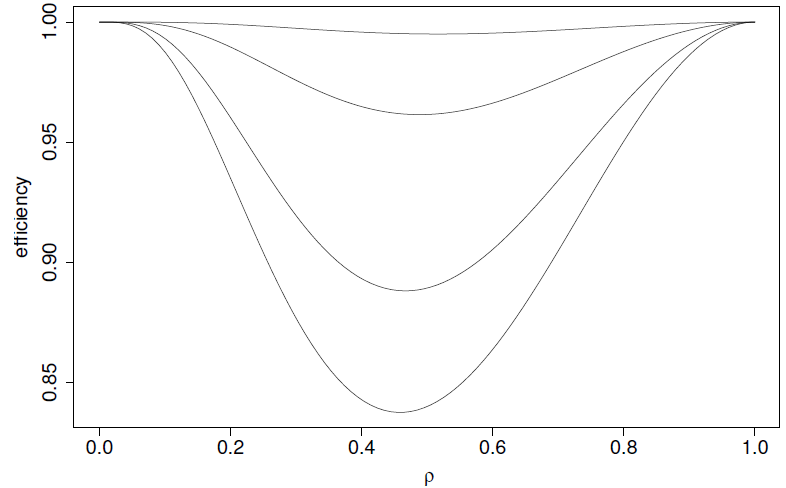
\epsfig{file=../FIGURES/Rei08-p8.eps, clip=, width=.5\textwidth}
    \end{tabular}
  \end{tabular}
  \]

  \bigskip\bigskip \pause
  \paragraph{Remark.} 
  ${\Var_\infty(\widehat{\rho}_L)}/{ \Var_\infty(\widehat{\rho}_{CL})} =
  1$ for $p=2$.

  }

%====================================================================
\subsection{Applications}
%====================================================================
\frame{\frametitle{Application: Stochastic Block Model} 

  \paragraph{Model.}
  \[
  \{Z_i\} \text{ iid } \Mcal(1; \pi), 
  \qquad
  \{Y_{ij}\} \text{ indep.}|Z, \quad (Y_{ij} | Z_i=k, Z_j=\ell) \sim
  \Bcal(\gamma_{k\ell}).
  \]

  \bigskip 
  \paragraph{Likelihood.} $\theta = (\pi, \gamma)$
  \[
  p(Y; \theta) = \sum_{z} p(Y, z; \theta)
  \]
  \ra Variational EM inference

  \bigskip \pause
  \paragraph{Composite log-likelihood.} \refer{AmM09}
  $$
  CL(Y; \theta) = \prod_{i \neq j \neq k} p(Y_{ij}, Y_{jk}, Y_{ik}; \theta).
  $$
  (Triplets of edges are required to guaranty identifiability.)
  }

%====================================================================
\frame{\frametitle{Application: Multivariate HMM} 

  \paragraph{Model.}
  \[
  \{Z_t = (Z_{it})\}_t \sim MC(\pi), 
  \qquad
  \{Y_{it}\} \text{ indep.}|Z, \quad (Y_{it} | Z_{it}=k) \sim
  \Fcal(\theta_k).
  \]

  \bigskip
  \paragraph{Composite likelihood.} \refer{GaS11}
  \[
  CL(Y; \theta) = \prod_{i \neq j} p(Y_i, Y_j; \theta)
  \]
  \pause \ra CL-EM algorithm 
  \begin{itemize}
  \item E-step: compute via forward-backward\footnote{\emphase{But is
    $\{(Z_{it}, Z_{jt})\}_t$ a Markov chain?}}    
    $$
    p(Z_i, Z_j | Y_i, Y_j; \theta);
    $$
  \item M-step: update
    $$
    \widehat{\theta} = \arg\max_\theta \sum_{i \neq j} \Esp\left[\log
    p(Y_i, Y_j, Z_i, Z_j; \theta) | Y_i, Y_j\right]
    $$
  \end{itemize}
  }

%====================================================================
%====================================================================
\section{Some Links?}
%====================================================================
\frame{\frametitle{Some Links?  \refer{Lyu11}} \pause

  \paragraph{Variational methods} 
  allow to deal with complex dependency structures by breaking down
  dependencies and provide efficient algorithms, but with almost no
  guaranty as for the parameter estimates.

  \bigskip\bigskip \pause
  \paragraph{Composite likelihood methods} 
  allow to deal with complex dependency structures by breaking down
  dependencies and provide guaranties as for the parameter estimates.

  \bigskip\bigskip \pause
  \paragraph{Question.} 
  Are variational methods like Mr Jourdain for composite likelihoods?
  % 
}

%====================================================================
\frame{\frametitle{KL contraction} 

  \paragraph{Definition \refer{Lyu11}.} 
  Denote $\Omega_d$ the set of all distributions over $\Rbb^d$. 
  \[
  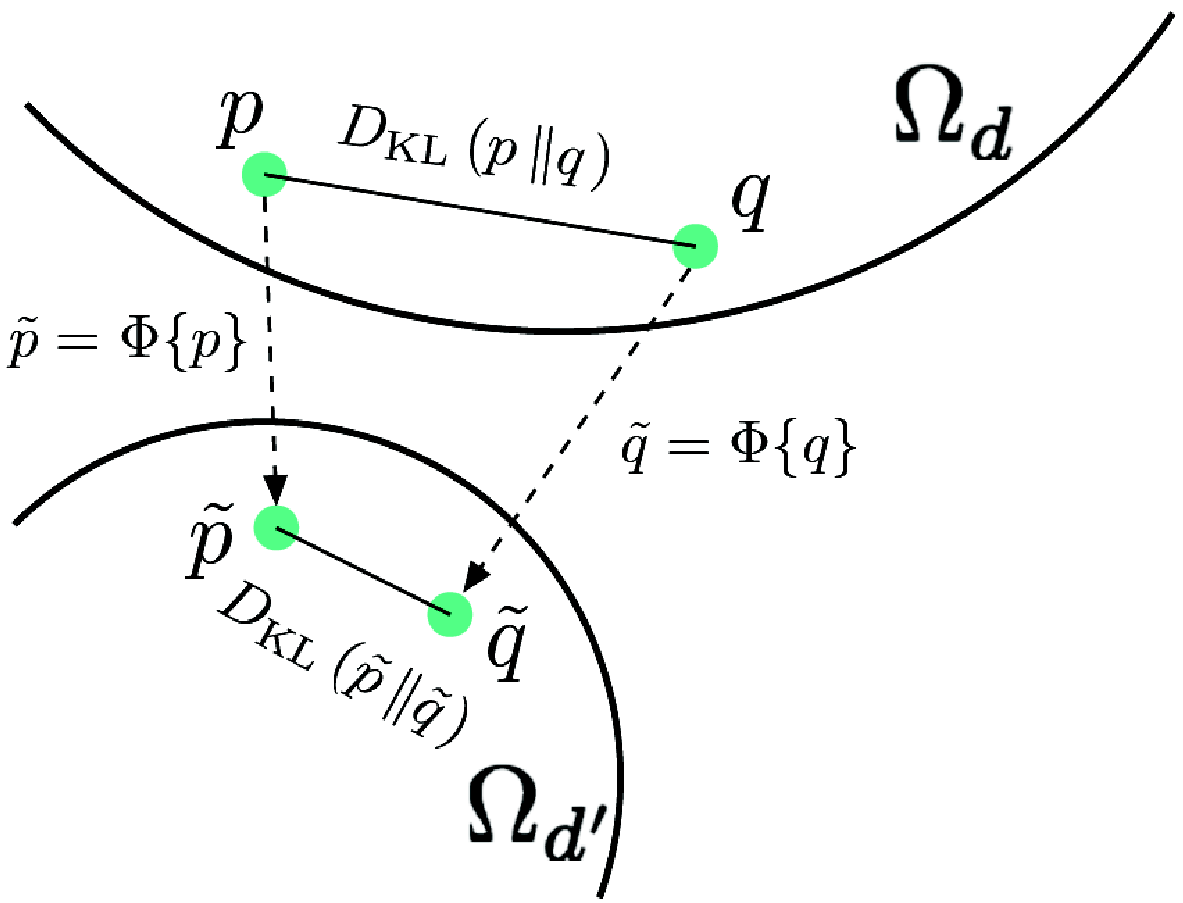
\epsfig{file=../FIGURES/Lyu11-Fig1.eps, width=.5\textwidth}
  \]
  $\Phi: \Omega_d \mapsto \Omega_{d'}$ is KL-contactant iff, $\exists
  \beta \geq 1$, $\forall p, q \in \Omega_d$: 
  $$
  \emphase{KL(p ||q) - \beta \; KL(\Phi\{p\} ||\Phi\{q\})} \geq 0.
  $$ 
}

%====================================================================
\frame{\frametitle{Examples of KL contraction} 

  For a given distribution $t(y|x)$
  \begin{itemize}
  \item \pause \emphase{Marginal distribution:} 
  $\displaystyle{\Phi^m_A\{p\}(x) = \int p(x) \dd x_{\setminus A}.}$ \\~ \pause
  \item \emphase{Conditional distribution:}
    $\displaystyle{\Phi^c_t\{p\}(y) = \int p(x) t(y|x) \dd x}.$ \\~ \pause
  \item \emphase{Marginal grafting:} (replaces $p_A(x_A)$ with $t_A(x_A)$)
    \[
    \Phi^g_{t, A}\{p\}(x) = p(x)
    \frac{t_A(x_A)}{p_A(x_A)} = t_A(x_A) p_{\setminus A
      |A}(x_{\setminus A}| x_A).
    \pause
    \]
  \item \emphase{Binary mixture:} $\displaystyle{\Phi^b_t\{p\}(x) =
    \pi t(x) + (1 - \pi) p(x).}$ \\~ \pause
  \item \emphase{Lumping} (= discretization): $\Scal = (S_1, \dots
    S_m)$ a partition of $\Rbb^d$,
    \[
    \Phi^\ell_\Scal\{p\}(i) = \int_{S_i} p(x) \dd x.
    \]
  \end{itemize}

}

%====================================================================
\frame{\frametitle{Possible use for inference} 

  \begin{enumerate}[Type I:]
  \item Avoid to compute normalizing constants, which can vanish in
    the difference 
    \begin{equation} \label{Eq:DiffKL}
      KL(p ||q_\theta) - \beta \; KL(\Phi\{p\}||\Phi\{q_\theta\})
    \end{equation} \\ \pause ~
  \item Define a easy-to-handle objective function based on a Taylor
    expansion of \eqref{Eq:DiffKL}. \\ \pause ~
  \item Use a set of contractions $(\Phi_1, \dots \Phi_K)$ to infer
    $\theta$ with
    \[
    \arg\min_\theta \sum_k w_k \left[KL(p||q_\theta) - \beta_k
      KL(\Phi_k\{p\}||\Phi_k\{q_\theta\}) \right].
    \]
  \end{enumerate}
  \refer{Lyu11}

  }

%====================================================================
\frame{\frametitle{Links with composite likelihoods} 

  \paragraph{Marginal contraction $\rightarrow$ Conditional composite 
    likelihood:}  
  For subsets $A_1, \dots A_K$, $p$ being the true distribution,
  \begin{align*}
    & \arg\min_\theta KL(p||q_\theta) - \sum_k w_k
    KL(\Phi_{A_k}^m\{p\}||\Phi_{A_k}^m\{q_\theta\}) \\ 
    %%
    = & \arg\min_\theta \int p(x) \log\frac{p(x)}{q(x; \theta)} \dd x
    - \sum_k w_k \int p(x) \log
    \frac{p_{A_k}(x_{A_k})}{q_{A_k}(x_{A_k}; \theta)} \dd x \\ 
    %%
    = & \arg\max_\theta \sum_k w_k \int p(x) \log \frac{q(x;
      \theta)}{q_{A_k}(x_{A_k}; \theta)} \dd x \qquad 
    \textcolor{grey}{\text{($p$ does not depend on $\theta$)}} \\
    %%
    = & \arg\max_\theta \sum_k w_k \int p(x) \log q_{\setminus A_k|
      A_k}(x_{\setminus A_k}|x_{A_k}; \theta) \dd x \\ 
    %%
    \approx & \arg\max_\theta \sum_k w_k \frac1n \sum_i \log
    q_{\setminus A_k| A_k}(x^i_{\setminus A_k}|x^i_{A_k}; \theta) \dd
    x \qquad \textcolor{grey}{\text{($p \rightarrow$ empirical dist.)}} 
  \end{align*}
}

%====================================================================
\frame{\frametitle{Links with composite likelihoods (cont'd)} 

  \paragraph{Marginal grafting $\rightarrow$ Marginal composite likelihood:} 
  \begin{align*}
    & \arg\min_\theta KL(p||q_\theta) - \sum_k w_k
    KL(\Phi_{p, A_k}^g\{p\}||\Phi_{p, A_k}^g\{q_\theta\}) \\ 
    %% 
    = & \arg\min_\theta \sum_k w_k
    KL(\Phi_{A_k}^m\{p\}||\Phi_{A_k}^m\{q_\theta\}) 
    \qquad \qquad \qquad \quad 
    \textcolor{grey}{\text{(cf Lemma 2)}}\\ 
    %%
    = & \arg\max_\theta \sum_k w_k \int p_{A_k}(x_{A_k}) \log
    q_{A_k}(x_{A_k}; \theta) \qquad 
    \textcolor{grey}{\text{($p$ does depend on $\theta$)}} \\
    %%
    \approx & \arg\max_\theta \sum_k w_k \frac1n \sum_i \log
    q_{A_k}(x^i_{A_k}; \theta) \qquad \qquad \quad \textcolor{grey}{\text{($p
        \rightarrow$ empirical dist.)}}
  \end{align*}
}

%====================================================================
\section{Conclusion}
%====================================================================
\frame{\frametitle{Conclusion: There is no conclusion} 

  \paragraph{Connexions do exist.} 
  Some variational approximations of the likelihood are actually
  composite likelihoods.

  \bigskip\bigskip \pause
  But is it the case of your favorite one?
  \[
  \min KL(q_\theta || p) \neq \min KL(p || q_\theta) \neq KL(p
  ||q_\theta) - \beta KL(\Phi\{p\}||\Phi\{q_\theta\}).
  \]

  \bigskip\bigskip \pause
  \paragraph{No nice example to show.}
  Not been able to derive the Godambe matrix for a given variational
  approximation. 
  \[
  \text{\ra Worth trying?}
  \]
  \refer{Lyu11}: '{\em While many non-ML learning methods covered in this
  work have been shown to be consistent individually, the unification
  based on the minimum KL contraction may provide a general condition
  for such asymptotic properties.}' ...

  }

%====================================================================
\section{References}
%====================================================================
\frame{\frametitle{References} 
{\tiny
  \bibliography{/media/donnees/Biblio/ARC,/media/donnees/Biblio/AST,/media/donnees/Biblio/SSB}
  \bibliographystyle{/media/donnees/LATEX/astats}
  %\bibliographystyle{plain}
  }}

%====================================================================
\section{Appendix}
%====================================================================
%====================================================================
\frame{\frametitle{Appendix: Symmetric multivariate Gaussian} 

  \paragraph{Covariance matrix.} 
  \begin{eqnarray*}
    \Rbf & = & (1-\rho) \Ibf + \rho \Jbf, \\
    \\
    \Rbf^{-1} & = & (1-\rho)^{-1} \left(\Ibf - \frac{\rho}{1 + (p-1)\rho} \Jbf
    \right), \\
    \\
  |\Rbf| & = & (1-\rho)^{p-1} [1 + (p-1) \rho]
  \end{eqnarray*}
}
  
%====================================================================
%====================================================================
\end{document}
%====================================================================
%====================================================================

%====================================================================
\frame{\frametitle{}
  }

  \vspace{-0.5cm}
  \begin{tabular}{cc}
    \hspace{-0.5cm}
    \begin{tabular}{p{.5\textwidth}}
    \end{tabular}
    &
    \hspace{-1cm}
    \begin{tabular}{p{.5\textwidth}}
    \end{tabular}
  \end{tabular}
